%pseudo code here defined with macro because else tabs won't reamin

\section{Introduction}

\begin{frame}
	\frametitle{What is a PID controller?}
	\small{
	\begin{definition}
		A \textbf{P}roportional \textbf{I}ntegral \textbf{D}eriviative controller is a control
		loop feedback mechanism (controller) widely used in process industry.
		\begin{figure}
			\centering
			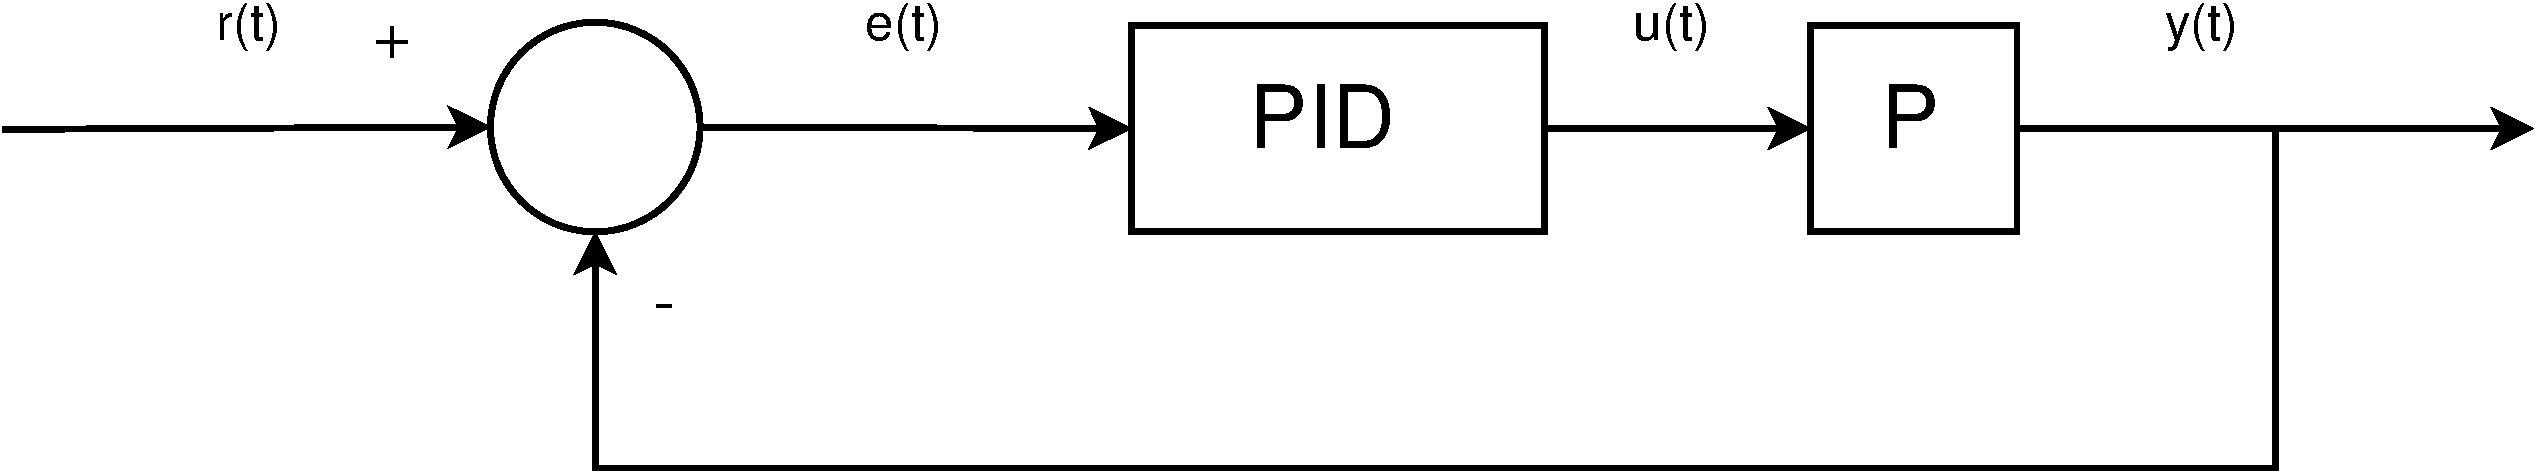
\includegraphics[width=0.8\linewidth]{img/PID}
		\end{figure}
		\vspace{-1em}
		Continuous-time text book equation:
		\begin{equation*}
			u(t) = 	\underbrace{\vphantom{\int^t_0e(\tau)d\tau}K_p e(t)}_\text{Proportional Action} 
					+ \underbrace{K_i\int^t_0e(\tau)d\tau}_\text{Integral Action} 
					+ \underbrace{\vphantom{\int^t_0e(\tau)d\tau} K_d \frac{de(t)}{dt}}_\text{Derivative Action}
		\end{equation*}
		\vspace{-1.5em}
		
	\end{definition}
	
	\textbf{Note:} More than 90\% of all closed loop controllers are PID.\\
}
\end{frame}

\begin{frame}
	\frametitle{What is a PID controller?}
	\small{
	\begin{itemize}
		\item \textbf{P}roportional action $u_p(t) = K_p e(t)$: Action depends on the instaneous value of the control error. 
			\begin{itemize}
				\pro Reduces rise time
				\con Reduces but \textbf{does not eliminate steady-state error}: Only when $K \rightarrow \infty , \text{error} \rightarrow 0$
				 (unless plant has pole(s) at $s=0$)
			\end{itemize}
		\item \textbf{I}ntegral action $u_i(t) =K_i\int_0^t e(\tau)d\tau$: Gives a controller output that is proportional to the accumulated error. Reacts on constant errors
			\begin{itemize}
				\pro  \textbf{Can eliminate steady state error} in some cases
				\con Makes transient response slower 
			\end{itemize}
	
		\item \textbf{D}erivative action $u_d(t) = K_d \frac{de(t)}{dt}$: Acts on the rate of change of the control error. 
			\begin{itemize}
				\pro Damping effect: reduces overshoot, improves transient response
				\con Sensitive for noise, amplifies it if present
			\end{itemize}
	\end{itemize}}
\end{frame}
\section{Analog and Digital formulations}

\begin{frame}
	\frametitle{Proportional Control}
	The continuous-time and discrete implementation are identical
	
	Continuous:
	\begin{equation*}
		u_p(t) = K_p e(t) \quad \rightarrow \quad \frac{U_p(s)}{E(s)} = K_p 
	\end{equation*}
	Discrete:
	\begin{equation*}
		u_p[k] = K_p e[k] \quad \rightarrow \quad \frac{U_p(z)}{E(z)} = K_p 
	\end{equation*}µ
	where e(t) or e[k] is the error signal.
\end{frame}

\begin{frame}
	\frametitle{Derrivative Control}
	Continuous:
	\begin{equation*}
		u_d(t) = K_d \frac{de(t)}{dt} \quad \rightarrow \quad \frac{U_d(s)}{E(s)} = K_d s 
	\end{equation*}
	Discrete (using \textbf{backward Euler}):
	\begin{equation*}
	u_d[k] = K_d \frac{ e[k] - e[k-1]}{T_s} \quad \rightarrow \quad \frac{U_d(z)}{E(z)} = K_d \frac{z - 1}{T_sz}
	\end{equation*}
	with $T_s$ the sampling time.

\end{frame}

\begin{frame}
	\frametitle{Integral Control}
	The continuous equation is:
	\begin{equation*}
		u_i(t) = K_i \int_0^t e(\tau)d\tau \quad \rightarrow \quad \frac{U_i(s)}{E(s)} = \frac{K_i}{s} 
	\end{equation*}
	Differentiating this gives :
	\begin{equation*}
		\dot{u_i} = K_i e(t)
	\end{equation*}
	
	Then applying backward Euler:
	\begin{equation*}
	u_i[k] = u[k-1] + K_i T e[k] \quad \rightarrow \quad \frac{U_i(z)}{E(z)} = K_i \frac{z T_s}{z - 1}
	\end{equation*}
	with $T_s$ the sampling time.
	
\end{frame}

\begin{frame}
	\frametitle{Digital formulation (conventional version)}
	\vspace{-1em}
	\small{
	\begin{block}{Digital PID controller (conventional version)}
			\vspace{-1em}
			%Difference equations
			\begin{align*}
			u[k] &= K_p e[k] + \frac{K_d}{T_s}(e[k] - e[k-1])+u_i[k] \\
			&\text{with } u_i[k] = u_i[k-1] + K_i T_s e[k]
			\end{align*}
			
			
			In z-domain:
			\begin{equation*}
			\frac{U(z)}{E(z)} = \textcolor{red}{K_p}  + \textcolor{red}{\frac{K_d}{T_s}}\frac{z-1}{z} + \textcolor{red}{K_i T_s}\frac{z}{z-1}
			\end{equation*}
			where $\frac{K_d}{T_s}$ and $K_iT_s$  are the new derivative and gains.
	\end{block}
	\begin{columns}
		\begin{column}{0.5 \textwidth}
			\begin{block}{Digital PI controller}
				$$\frac{U(z)}{E(z)} = K_p + K_i T \frac{z}{z-1} $$
			\end{block}
		\end{column}
		\begin{column}{0.5 \textwidth}
			\begin{block}{Digital PD controller}
				$$\frac{U(z)}{E(z)} = K_p + \frac{K_d}{T}\frac{z-1}{z} $$
			\end{block}
		\end{column}
	\end{columns}}
	%\vspace{1em}
	 
\end{frame}

\begin{frame}
	\frametitle{Alternative Digital PID controller}
	We can also discretize using the \textbf{bilinear transformation}:
	\begin{align*}
		\frac{U(z)}{E(z)} &=  
				\left. K_p + \frac{K_i}{s} + K_d s \right|_
							{s=\frac{2}{T}\left( \frac{z-1}{z+1}\right)}  \\
			&= K_p + \frac{K_iT(z + 1)}{2(z-1)} + \frac{2K_d(z-1)}{T(z+1)} \\
			&= \frac{\alpha_2 z^2 + \alpha_1 z + \alpha_0}{(z-1)(z+1)}
	\end{align*}
	
	where $\alpha_2, \alpha_1, \alpha_0$ are design parameters.
	
\end{frame}
\begin{frame}
	\begin{figure}
\centering
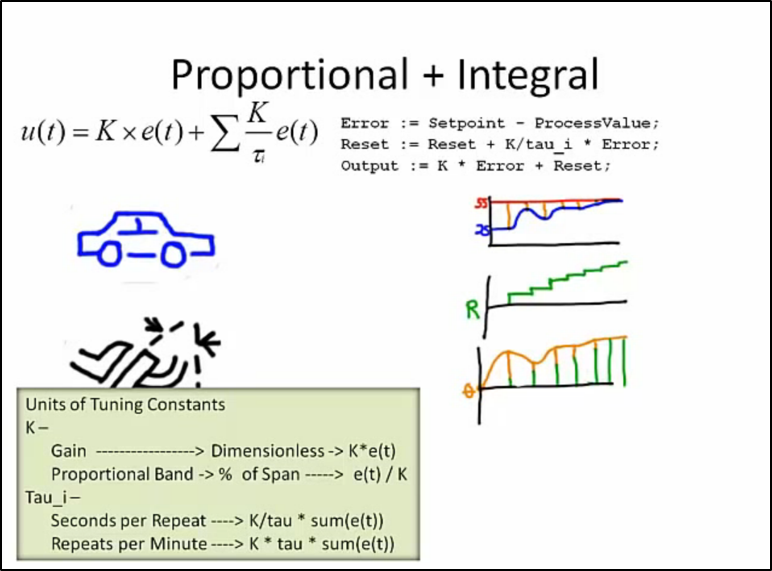
\includegraphics[width=0.7\linewidth]{img/PID_video}

\end{figure}

	\url{https://www.youtube.com/watch?v=JEpWlTl95Tw}
\end{frame}
\begin{frame}
	\frametitle{Alterantive Derivative Action(Continous time)}
		\begin{columns}
			\begin{column}{0.7\linewidth}
				Imagine a jumping set point or rapidly changing signal. 
				This results in a theoretically infinite, practically very large response of
				the derivative term.  
			\end{column}
			\begin{column}{0.3\linewidth}
				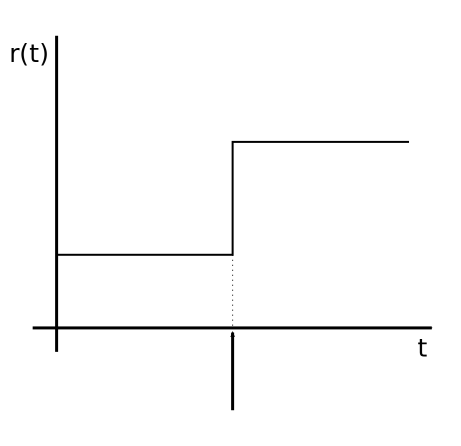
\includegraphics[width=\linewidth]{img/piecewise-setpoint}
			\end{column}
		\end{columns}
		$\Rightarrow$ Add a low-pass filter to the derivative term:
		\begin{equation*}
			\frac{U_d(s)}{E(s)} = \frac{K_d s}{1+s\tau}
		\end{equation*}
		With $s=j\omega$, breakpoint at $\omega=1/\tau$. This prevents amplification of high frequencies. 
	
\end{frame}

\begin{frame}
	\frametitle{Alterantive Derivative Action(Continous time)}
	\begin{equation*}
		\frac{U_d(s)}{E(s)} = \frac{K_d s}{1+s\tau}
	\end{equation*}
	
	Further $e(t)$ is replaced by $c\cdot r(t)-y(t)$ with c the set point weighting, which is often set to zero to further reduce immediate influence of a sudden set point jump. 
	
	In time domain:
	
	\begin{equation*}
		u_d(t) = -\tau\frac{du_d}{dt} + K_d(c\cdot r(t)-y(t))
	\end{equation*}
	
	This can also be discretized, but the bilinear method then introduces \emph{ringing}, i.e. large oscillations in transient response.
\end{frame}
\section{Implementation Examples}

\begin{frame}
	\frametitle{Analog Implementation}
	The key building block is the operational amplifier (op-amp).
	\begin{columns}
		\begin{column}{0.7 \textwidth}
			\begin{figure}
				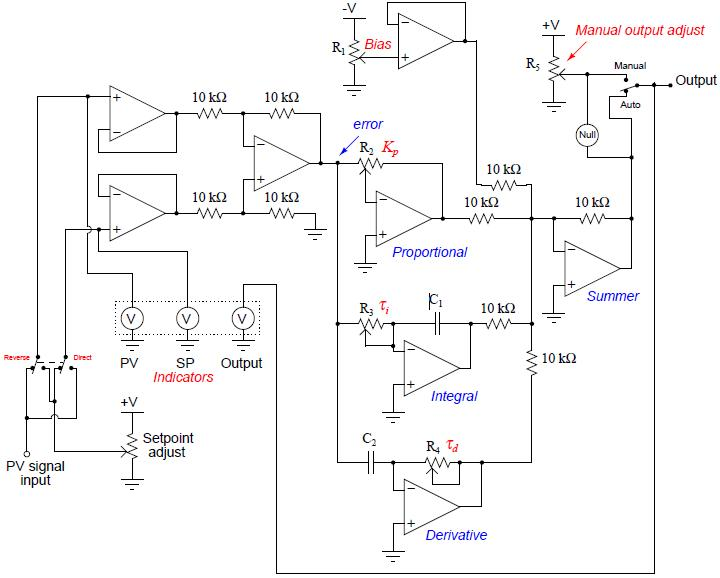
\includegraphics[width=1\linewidth]{img/Principles_of_Feedback_Control_Fig_079}
			\end{figure}
		\end{column}
		\begin{column}{0.3 \textwidth}
			\footnotesize{
				\begin{itemize}
					\item PV - Process Variable $y(t)$
					\item SP - Set Point $r(t)$
					\item Output - Control action $u(t)$
				\end{itemize}
			}
		\end{column}
	\end{columns}
\end{frame}

\begin{frame}
	\frametitle{Analog Implementation}
	\begin{columns}
		\begin{column}{0.3\linewidth}
			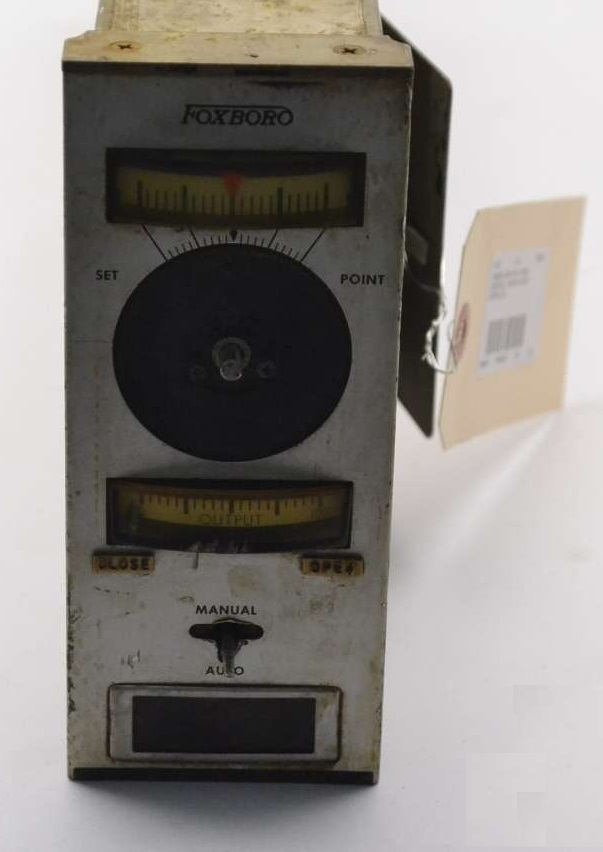
\includegraphics[height=0.6\textheight]{img/FB2a}
		\end{column}
		\begin{column}{0.2\linewidth}
			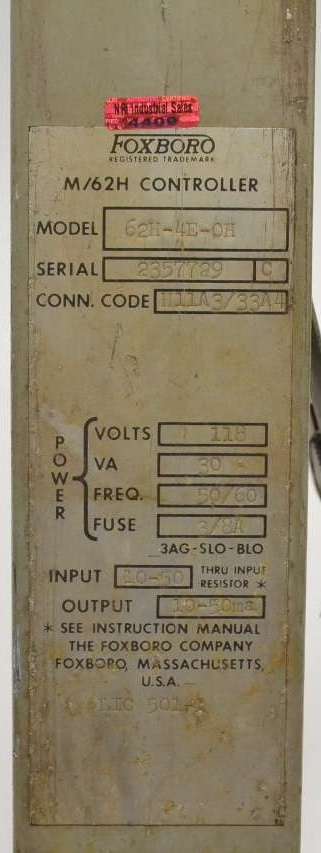
\includegraphics[height=0.6\textheight]{img/fb3a}
		\end{column}
		\begin{column}{0.5\linewidth}
			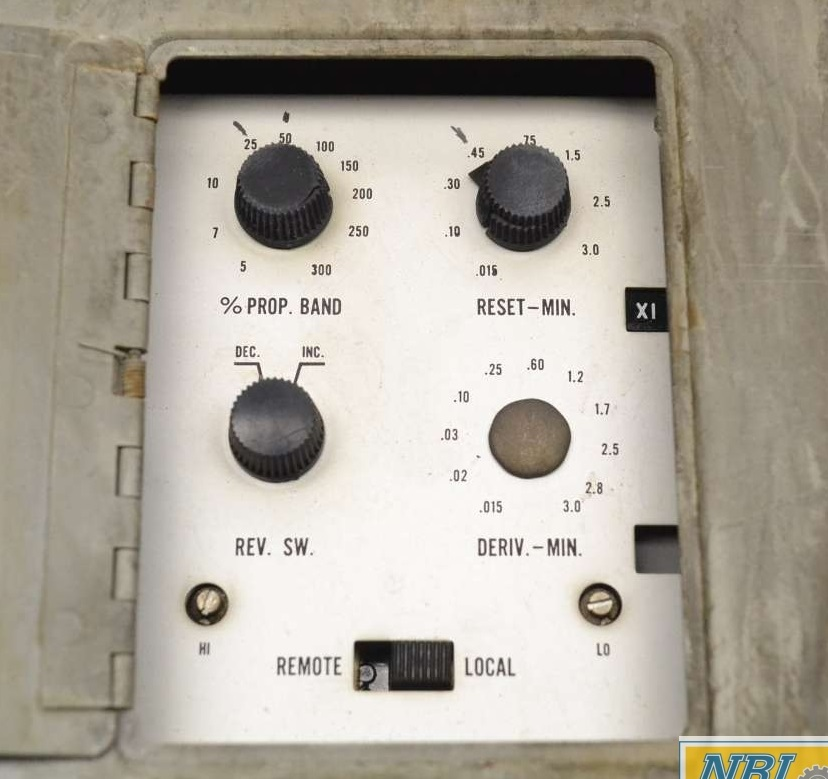
\includegraphics[height=0.6\textheight]{img/fb4}
		\end{column}
	\end{columns}
	\begin{center}
		\textbf{FOXBORO 62H-4E-OH M/62H}
	\end{center}
\end{frame}
\begin{frame}{Analog PI Motor Speed Control}
	\begin{figure}
		\centering
		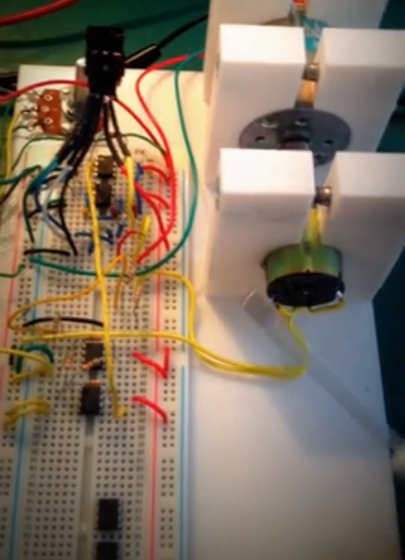
\includegraphics[width=0.4\linewidth]{img/feedback_motor}
	\end{figure}
	\url{https://youtu.be/6W3PLiVIcmE}
\end{frame}
\begin{frame}[fragile]
	\frametitle{Digital Implementation}
	\small{
	The difference equations are typically implemented in a micro controller or FPGA (field-programmable gate array):
		\begin{align*}
		u[k] &= K_p e[k] + \frac{K_d}{T}(e[k] - e[k-1])+u_i[k] \\
		&\text{with } u_i[k] = u_i[k-1] + K_i T e[k]
		\end{align*}
	Steps to be implemented:}
\begin{lstlisting}[
basicstyle=\scriptsize
]
previous_error = 0
integral = 0
Start:
	error = setpoint - measured_value
	proportional = K_P * error
	integral = integral + K_i*sampling_time*error
	derivative = K_d*(error-previous_error)/sampling_time
	output = proportional + integral + derivative
	previous_error = error
	wait(sampling_time)
	goto Start
	\end{lstlisting}
%	\begin{enumerate}
%		\item Wait for clock interrupt
%		\item Read analog input
%		\item Compute control signal
%		\item Set analog output
%		\item Update controller variables
%		\item Go to 1
%	\end{enumerate}
\end{frame}

\begin{frame}
	\frametitle{Digital Implementation Example}
	\begin{columns}
		\begin{column}{0.5\linewidth}
			\centering PLC with a digital PID module:
			
			\vspace{1em}
			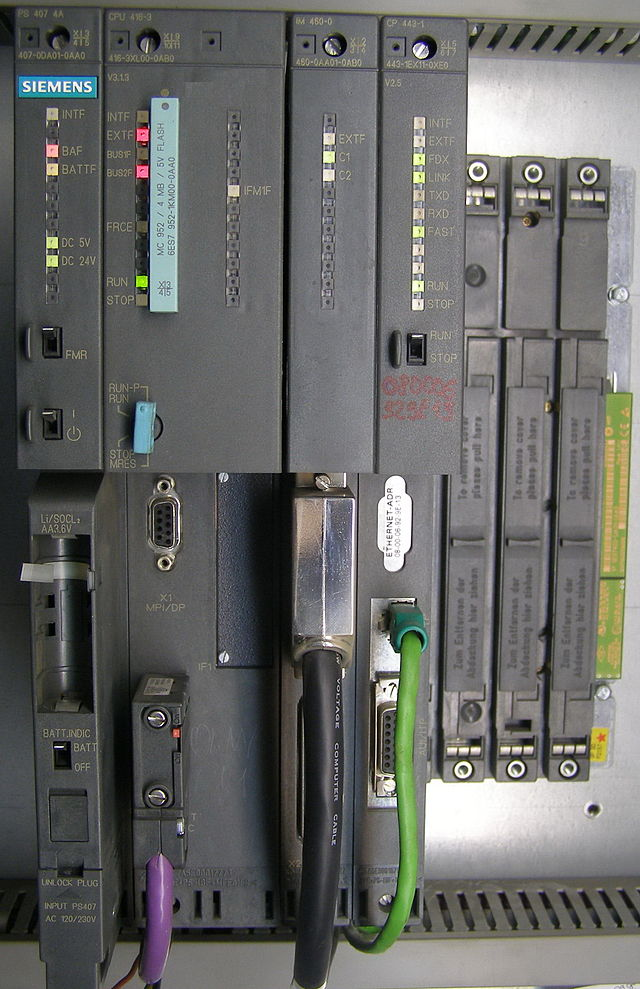
\includegraphics[height=0.7\textheight]{img/640px-Siemens_Simatic_S7-416-3}
		\end{column}
		\begin{column}{0.5\linewidth}
			\centering Digital PID's:
			\vspace{1em}
			\begin{columns}
				\begin{column}{0.4\linewidth}
					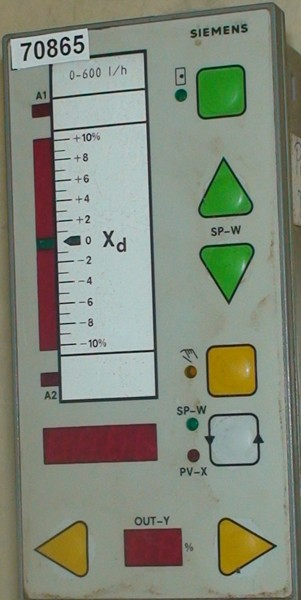
\includegraphics[height=0.7\textheight]{img/278}

				\end{column}
				\begin{column}{0.6\linewidth}
					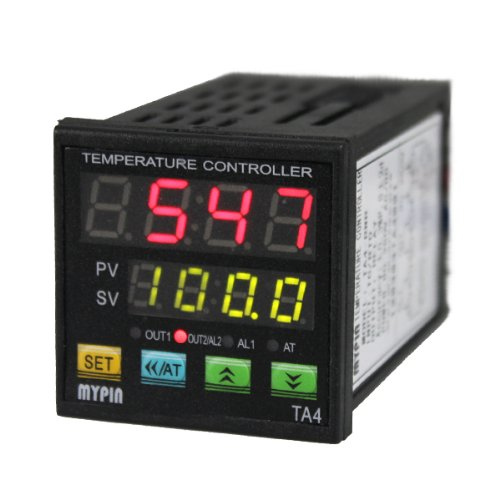
\includegraphics[height=0.4\textheight]{img/41LH64+SGWL}

				\end{column}
			\end{columns}
		\end{column}
	\end{columns}
\end{frame}
\begin{frame}{PLC}
	\textbf{P}rogrammable \textbf{L}ogic \textbf{C}ontroller is a digital computer used for automation in the process industry. 
	\begin{columns}
		\begin{column}{0.5\textwidth}
			\begin{figure}
				\centering
				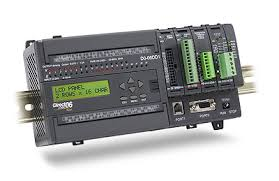
\includegraphics[width=0.7\linewidth]{img/PLC_1}
			\end{figure}

		\end{column}
		\begin{column}{0.5\textwidth}
\begin{figure}
\centering
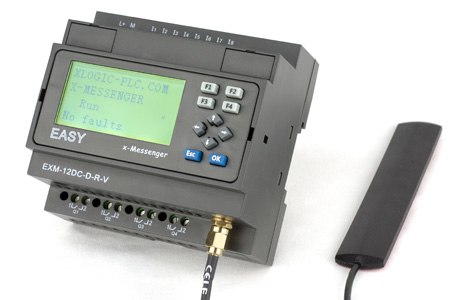
\includegraphics[width=0.7\linewidth]{img/PLC_2}

\end{figure}

		\end{column}
	\end{columns}
	
\end{frame}
\begin{frame}{What is a PLC? Basics of PLCs}
	\begin{figure}
\centering
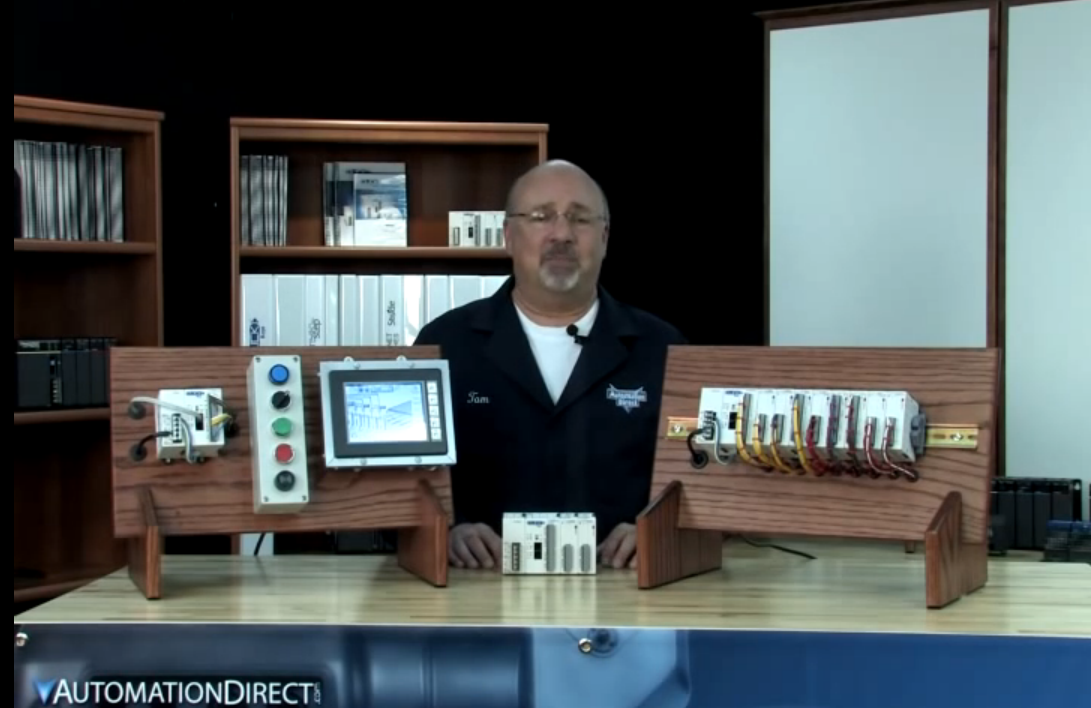
\includegraphics[width=0.7\linewidth]{img/what_is_a_plc}
\end{figure}

	\url{https://youtu.be/iWgHqqunsyE}
\end{frame}
\section{PID Tuning}

\begin{frame}
	Effects of adjusting the parameters $K_p, K_i, K_d$:
	\vspace{1em}
	\frametitle{Manual Tuning}
	{
	\small
	\begin{tabular}{c | c | c | c | c }
		PID gains	&	Rise Time 	&	Overshoot	&	Setlling time	&	Steady-State error \\
		\hline
		$K_p \uparrow$ & Decrease	&	Increase	&	Small Change	&	Decrease \\
		$K_i \uparrow$ & Decrease	&	Increase	&	Increase		&	Eliminate \\
		$K_d \uparrow$ & Small change &	Decrease	&	Decrease		&	No change \\
	\end{tabular}
	}
	\vspace{1em}
	
	\textbf{Note:} Changing one parameter can influence the effect of the other two. Use this table only as an indication.
\end{frame}

\begin{frame}
	\frametitle{Manual Tuning}
	The controller can be tuned while connected to the plant. Following routine can be used:
	\begin{enumerate}
		\item Set $K_i$ and $K_d$ equal to 0
		\item Increase $K_p$ until you observe that the step response is fast enough and the steady-state error in small
		\item Start adding some integral action in order to get rid of the steady state error. Keep in mind that too much $K_i$ can cause instability!
		\item Add some derivative action in order to quickly react to disturbance and/or dampen the response
		
	\end{enumerate}
\end{frame}


\begin{frame}
	\frametitle{Heuristic Methods: Ziegler-Nichols tunig rule}
		This method relies on empirically determining two parameters of the system:
		\begin{enumerate}
			\item Set the integral and derivative gains to 0
			\item Increase the proportional gain $K_p$ until the output of the control loop starts oscillating with at constant amplitude. The value of $K_p$ at this point is referred to as ultimate gain $K_u \triangleq K_p$
			\item Measure the period of the oscillations $T_u$ at the output
			\item Adjust the controller parameters according the table on the next slide.
		\end{enumerate}
\end{frame}

\begin{frame}
	\frametitle{Heuristic Methods: Ziegler-Nichols tunig rule}
	With $K_u$ and $T_u$ determined like in the previous slide, a starting point for the parameters can be determined:
	\vspace{1em}
	
	\begin{tabular}{c | c | c | c}
		Control Type	&	$K_p$		&	$K_i$			&	$K_d$ 	\\
		\hline
		P				&	$0.5K_u$	&	-				&	-		\\
		PI				&	$0.45K_u$	&	$1.2K_p/T_u$		&	-		\\
		PD				&	$0.8K_u$	&	-				&	$K_pT_u/8$ \\
		PID				&	$0.6K_u$	&	$2K_p/T_u$		&	$K_pT_u/8$ \\
		Pessen Integral Rule & $0.7K_u$ &	$2.5K_p/T_u$	&	$3K_pT_u/20$\\
		Some overshoot	&	$0.33K_u$	&	$2K_p/T_u$		&	$K_pT_u/3$	\\
		No overshoot	&	$0.2K_u$	&	$2K_p/T_u$		&	$K_pT_u/3$	\\
	\end{tabular}
\end{frame}
\begin{frame}{Heuristic Methods: Ziegler-Nichols tuning rule(example)}
	\vspace{-1em}
	\footnotesize{
	\begin{example}
		Consider a plant with a given model:\\
		\vspace{-0.5em}
			$$ P(s) = \frac{1}{(s+1)^3} $$\\
			\vspace{-0.7em}
			\begin{itemize}
				\item We compute the critical gain $K_c$. This is the value of $K_p$ for which $\angle (K_p P(s)) = - 180^\circ$. On the Nyquist plot this the value of $K_p$ for which $K_p P(s)$ passes through $(-1,0)$.\\
			\end{itemize}
				\vspace{-1.5em}
				\begin{columns}
					\begin{column}{0.5 \textwidth}
							\begin{align*}
							K_cP(j\omega_c) &= -1 \\ \Leftrightarrow K_c &= 	-(j\omega_c + 1)^3 \\
								& = (3\omega_c^2-1)+j(\omega_c^3 - 3\omega_c)
							\end{align*}
								\vspace{-1.5em}
								$$ \omega_c^3-3\omega_c = 0 \Rightarrow \omega_c = \sqrt{3}$$\\
								\vspace{-1.5em}
								$$K_c = 8, T_u = \frac{2\pi}{\omega} = 3.628$$\\
								\vspace{-1.5em}
								$$K_p = 4.8, K_I = 0.551  K_p, K_d =  0.45 K_p$$
						
					\end{column}
					\begin{column}{0.4 \textwidth}
\begin{figure}
\centering
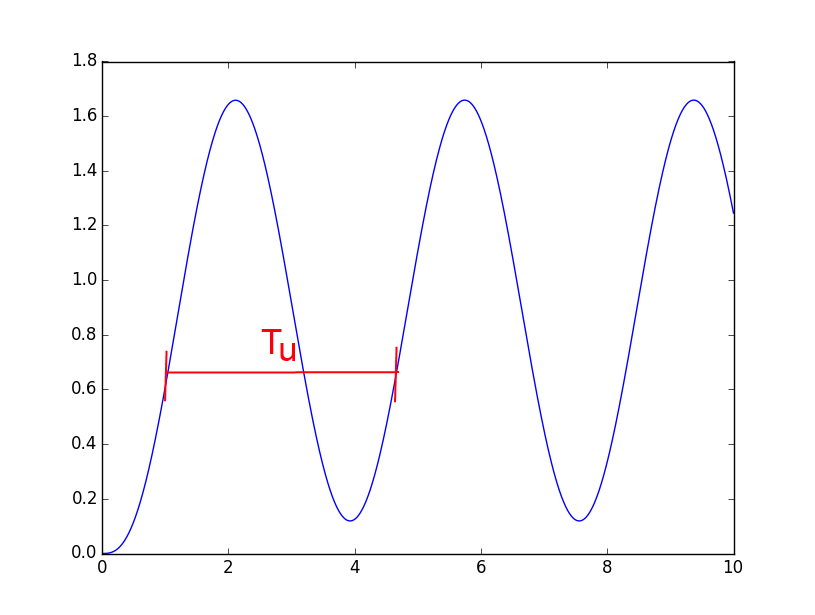
\includegraphics[width=1\linewidth]{img/Z_N_PID_example}
\end{figure}

					\end{column}
				\end{columns}
			
	\end{example}}
\end{frame}
\begin{frame}
	\small{
	\frametitle{Numeriacal Optimization Methods}
	The tuning of a PID controller is posed as a constrained optimization problem. 
	\begin{itemize}
			\item For a given set of parameters $K_p$, $K_i$ and $K_d$ run a simulation of the closed-loop system, and compute some performance parameters (e.g. setting time, rise time, etc.) and a performance index.
			\item Optimize the performance index over the three PID gains.
	\end{itemize}}
\begin{figure}

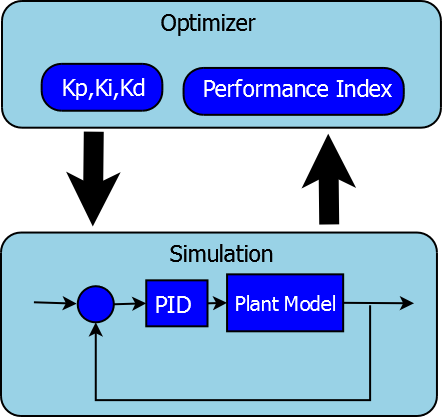
\includegraphics[width=0.3\linewidth]{img/PID_1}
\end{figure}

	
\end{frame}
\begin{frame}{Some Software Tools}
	\small{
	\begin{tabular}{|p{3cm}|p{7cm}|}
		\hline Software Tool  & Brief Description  \\ 
		\hline pidtool / pidTuner
		 & It is a Matlab tool to interactively design a SISO PID controller in the feed-forward path of single-loop, unity-feedback control configuration \\ 
		\hline Pidpy
		 & It is a modular PID control library for python that supports PID auto tuning. \url{https://pypi.python.org/pypi/pypid/}
		  \\ 
		\hline INCA PID Tuner
		 & It is a commercial tuning tool developed by IPCOS. It has a vast library of PID structures for DCS and PLC  Systems including Siemens, ABB, Honeywell, Emerson, etc. \url{http://www.ipcos.com/advancedprocesscontrol/advanced-process-control/pid-tuning-software/inca-pid-tuning/}
		   \\ 
		\hline 
	\end{tabular}}
\end{frame}
\begin{frame}{pidtool /pidTuner - Demo}
	\begin{figure}
\centering
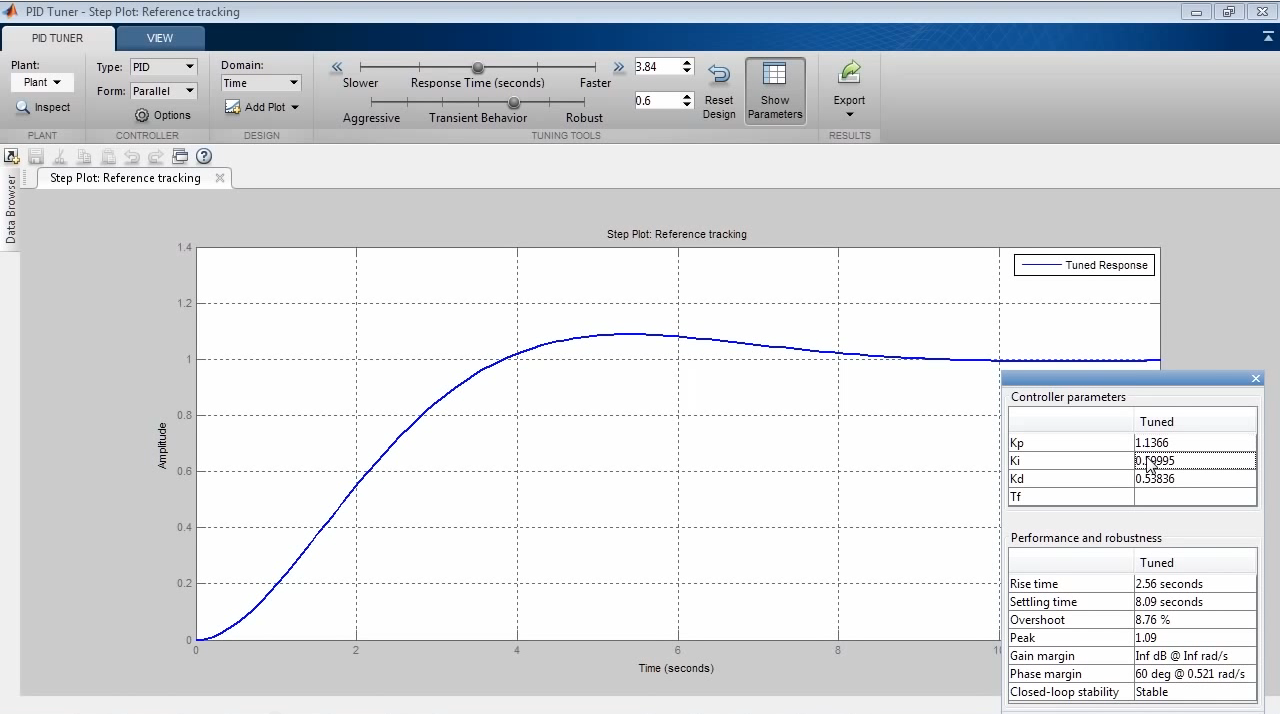
\includegraphics[width=0.7\linewidth]{img/pid_tool}

\end{figure}
\url{https://www.youtube.com/watch?v=2tKe0caUv1I}
\end{frame}
\begin{frame}{INCA PID Tuner – Demo}
	\begin{figure}
\centering
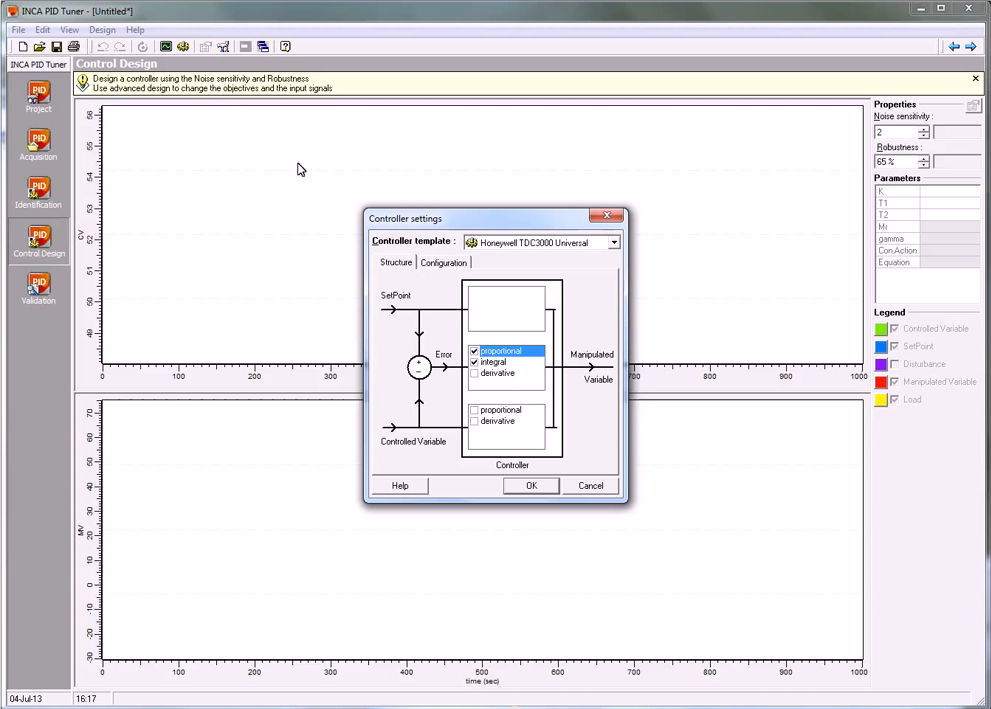
\includegraphics[width=0.7\linewidth]{img/inca_tunner}
\end{figure}
\url{https://www.youtube.com/watch?v=XH2bkq1URSg}
\end{frame}